
% Default to the notebook output style

    


% Inherit from the specified cell style.




    
\documentclass[11pt]{article}

    
    
    \usepackage[T1]{fontenc}
    % Nicer default font (+ math font) than Computer Modern for most use cases
    \usepackage{mathpazo}

    % Basic figure setup, for now with no caption control since it's done
    % automatically by Pandoc (which extracts ![](path) syntax from Markdown).
    \usepackage{graphicx}
    % We will generate all images so they have a width \maxwidth. This means
    % that they will get their normal width if they fit onto the page, but
    % are scaled down if they would overflow the margins.
    \makeatletter
    \def\maxwidth{\ifdim\Gin@nat@width>\linewidth\linewidth
    \else\Gin@nat@width\fi}
    \makeatother
    \let\Oldincludegraphics\includegraphics
    % Set max figure width to be 80% of text width, for now hardcoded.
    \renewcommand{\includegraphics}[1]{\Oldincludegraphics[width=.8\maxwidth]{#1}}
    % Ensure that by default, figures have no caption (until we provide a
    % proper Figure object with a Caption API and a way to capture that
    % in the conversion process - todo).
    \usepackage{caption}
    \DeclareCaptionLabelFormat{nolabel}{}
    \captionsetup{labelformat=nolabel}

    \usepackage{adjustbox} % Used to constrain images to a maximum size 
    \usepackage{xcolor} % Allow colors to be defined
    \usepackage{enumerate} % Needed for markdown enumerations to work
    \usepackage{geometry} % Used to adjust the document margins
    \usepackage{amsmath} % Equations
    \usepackage{amssymb} % Equations
    \usepackage{textcomp} % defines textquotesingle
    % Hack from http://tex.stackexchange.com/a/47451/13684:
    \AtBeginDocument{%
        \def\PYZsq{\textquotesingle}% Upright quotes in Pygmentized code
    }
    \usepackage{upquote} % Upright quotes for verbatim code
    \usepackage{eurosym} % defines \euro
    \usepackage[mathletters]{ucs} % Extended unicode (utf-8) support
    \usepackage[utf8x]{inputenc} % Allow utf-8 characters in the tex document
    \usepackage{fancyvrb} % verbatim replacement that allows latex
    \usepackage{grffile} % extends the file name processing of package graphics 
                         % to support a larger range 
    % The hyperref package gives us a pdf with properly built
    % internal navigation ('pdf bookmarks' for the table of contents,
    % internal cross-reference links, web links for URLs, etc.)
    \usepackage{hyperref}
    \usepackage{longtable} % longtable support required by pandoc >1.10
    \usepackage{booktabs}  % table support for pandoc > 1.12.2
    \usepackage[inline]{enumitem} % IRkernel/repr support (it uses the enumerate* environment)
    \usepackage[normalem]{ulem} % ulem is needed to support strikethroughs (\sout)
                                % normalem makes italics be italics, not underlines
    

    
    
    % Colors for the hyperref package
    \definecolor{urlcolor}{rgb}{0,.145,.698}
    \definecolor{linkcolor}{rgb}{.71,0.21,0.01}
    \definecolor{citecolor}{rgb}{.12,.54,.11}

    % ANSI colors
    \definecolor{ansi-black}{HTML}{3E424D}
    \definecolor{ansi-black-intense}{HTML}{282C36}
    \definecolor{ansi-red}{HTML}{E75C58}
    \definecolor{ansi-red-intense}{HTML}{B22B31}
    \definecolor{ansi-green}{HTML}{00A250}
    \definecolor{ansi-green-intense}{HTML}{007427}
    \definecolor{ansi-yellow}{HTML}{DDB62B}
    \definecolor{ansi-yellow-intense}{HTML}{B27D12}
    \definecolor{ansi-blue}{HTML}{208FFB}
    \definecolor{ansi-blue-intense}{HTML}{0065CA}
    \definecolor{ansi-magenta}{HTML}{D160C4}
    \definecolor{ansi-magenta-intense}{HTML}{A03196}
    \definecolor{ansi-cyan}{HTML}{60C6C8}
    \definecolor{ansi-cyan-intense}{HTML}{258F8F}
    \definecolor{ansi-white}{HTML}{C5C1B4}
    \definecolor{ansi-white-intense}{HTML}{A1A6B2}

    % commands and environments needed by pandoc snippets
    % extracted from the output of `pandoc -s`
    \providecommand{\tightlist}{%
      \setlength{\itemsep}{0pt}\setlength{\parskip}{0pt}}
    \DefineVerbatimEnvironment{Highlighting}{Verbatim}{commandchars=\\\{\}}
    % Add ',fontsize=\small' for more characters per line
    \newenvironment{Shaded}{}{}
    \newcommand{\KeywordTok}[1]{\textcolor[rgb]{0.00,0.44,0.13}{\textbf{{#1}}}}
    \newcommand{\DataTypeTok}[1]{\textcolor[rgb]{0.56,0.13,0.00}{{#1}}}
    \newcommand{\DecValTok}[1]{\textcolor[rgb]{0.25,0.63,0.44}{{#1}}}
    \newcommand{\BaseNTok}[1]{\textcolor[rgb]{0.25,0.63,0.44}{{#1}}}
    \newcommand{\FloatTok}[1]{\textcolor[rgb]{0.25,0.63,0.44}{{#1}}}
    \newcommand{\CharTok}[1]{\textcolor[rgb]{0.25,0.44,0.63}{{#1}}}
    \newcommand{\StringTok}[1]{\textcolor[rgb]{0.25,0.44,0.63}{{#1}}}
    \newcommand{\CommentTok}[1]{\textcolor[rgb]{0.38,0.63,0.69}{\textit{{#1}}}}
    \newcommand{\OtherTok}[1]{\textcolor[rgb]{0.00,0.44,0.13}{{#1}}}
    \newcommand{\AlertTok}[1]{\textcolor[rgb]{1.00,0.00,0.00}{\textbf{{#1}}}}
    \newcommand{\FunctionTok}[1]{\textcolor[rgb]{0.02,0.16,0.49}{{#1}}}
    \newcommand{\RegionMarkerTok}[1]{{#1}}
    \newcommand{\ErrorTok}[1]{\textcolor[rgb]{1.00,0.00,0.00}{\textbf{{#1}}}}
    \newcommand{\NormalTok}[1]{{#1}}
    
    % Additional commands for more recent versions of Pandoc
    \newcommand{\ConstantTok}[1]{\textcolor[rgb]{0.53,0.00,0.00}{{#1}}}
    \newcommand{\SpecialCharTok}[1]{\textcolor[rgb]{0.25,0.44,0.63}{{#1}}}
    \newcommand{\VerbatimStringTok}[1]{\textcolor[rgb]{0.25,0.44,0.63}{{#1}}}
    \newcommand{\SpecialStringTok}[1]{\textcolor[rgb]{0.73,0.40,0.53}{{#1}}}
    \newcommand{\ImportTok}[1]{{#1}}
    \newcommand{\DocumentationTok}[1]{\textcolor[rgb]{0.73,0.13,0.13}{\textit{{#1}}}}
    \newcommand{\AnnotationTok}[1]{\textcolor[rgb]{0.38,0.63,0.69}{\textbf{\textit{{#1}}}}}
    \newcommand{\CommentVarTok}[1]{\textcolor[rgb]{0.38,0.63,0.69}{\textbf{\textit{{#1}}}}}
    \newcommand{\VariableTok}[1]{\textcolor[rgb]{0.10,0.09,0.49}{{#1}}}
    \newcommand{\ControlFlowTok}[1]{\textcolor[rgb]{0.00,0.44,0.13}{\textbf{{#1}}}}
    \newcommand{\OperatorTok}[1]{\textcolor[rgb]{0.40,0.40,0.40}{{#1}}}
    \newcommand{\BuiltInTok}[1]{{#1}}
    \newcommand{\ExtensionTok}[1]{{#1}}
    \newcommand{\PreprocessorTok}[1]{\textcolor[rgb]{0.74,0.48,0.00}{{#1}}}
    \newcommand{\AttributeTok}[1]{\textcolor[rgb]{0.49,0.56,0.16}{{#1}}}
    \newcommand{\InformationTok}[1]{\textcolor[rgb]{0.38,0.63,0.69}{\textbf{\textit{{#1}}}}}
    \newcommand{\WarningTok}[1]{\textcolor[rgb]{0.38,0.63,0.69}{\textbf{\textit{{#1}}}}}
    
    
    % Define a nice break command that doesn't care if a line doesn't already
    % exist.
    \def\br{\hspace*{\fill} \\* }
    % Math Jax compatability definitions
    \def\gt{>}
    \def\lt{<}
    % Document parameters
    \title{COMS3007: Machine Learning Assignment}
    \author{    Tristan Nagan: 1484720 \and Marc Marsden: 1437889 \and Lehyendran Govender: 1106458}
    
    
    

    % Pygments definitions
    
\makeatletter
\def\PY@reset{\let\PY@it=\relax \let\PY@bf=\relax%
    \let\PY@ul=\relax \let\PY@tc=\relax%
    \let\PY@bc=\relax \let\PY@ff=\relax}
\def\PY@tok#1{\csname PY@tok@#1\endcsname}
\def\PY@toks#1+{\ifx\relax#1\empty\else%
    \PY@tok{#1}\expandafter\PY@toks\fi}
\def\PY@do#1{\PY@bc{\PY@tc{\PY@ul{%
    \PY@it{\PY@bf{\PY@ff{#1}}}}}}}
\def\PY#1#2{\PY@reset\PY@toks#1+\relax+\PY@do{#2}}

\expandafter\def\csname PY@tok@w\endcsname{\def\PY@tc##1{\textcolor[rgb]{0.73,0.73,0.73}{##1}}}
\expandafter\def\csname PY@tok@c\endcsname{\let\PY@it=\textit\def\PY@tc##1{\textcolor[rgb]{0.25,0.50,0.50}{##1}}}
\expandafter\def\csname PY@tok@cp\endcsname{\def\PY@tc##1{\textcolor[rgb]{0.74,0.48,0.00}{##1}}}
\expandafter\def\csname PY@tok@k\endcsname{\let\PY@bf=\textbf\def\PY@tc##1{\textcolor[rgb]{0.00,0.50,0.00}{##1}}}
\expandafter\def\csname PY@tok@kp\endcsname{\def\PY@tc##1{\textcolor[rgb]{0.00,0.50,0.00}{##1}}}
\expandafter\def\csname PY@tok@kt\endcsname{\def\PY@tc##1{\textcolor[rgb]{0.69,0.00,0.25}{##1}}}
\expandafter\def\csname PY@tok@o\endcsname{\def\PY@tc##1{\textcolor[rgb]{0.40,0.40,0.40}{##1}}}
\expandafter\def\csname PY@tok@ow\endcsname{\let\PY@bf=\textbf\def\PY@tc##1{\textcolor[rgb]{0.67,0.13,1.00}{##1}}}
\expandafter\def\csname PY@tok@nb\endcsname{\def\PY@tc##1{\textcolor[rgb]{0.00,0.50,0.00}{##1}}}
\expandafter\def\csname PY@tok@nf\endcsname{\def\PY@tc##1{\textcolor[rgb]{0.00,0.00,1.00}{##1}}}
\expandafter\def\csname PY@tok@nc\endcsname{\let\PY@bf=\textbf\def\PY@tc##1{\textcolor[rgb]{0.00,0.00,1.00}{##1}}}
\expandafter\def\csname PY@tok@nn\endcsname{\let\PY@bf=\textbf\def\PY@tc##1{\textcolor[rgb]{0.00,0.00,1.00}{##1}}}
\expandafter\def\csname PY@tok@ne\endcsname{\let\PY@bf=\textbf\def\PY@tc##1{\textcolor[rgb]{0.82,0.25,0.23}{##1}}}
\expandafter\def\csname PY@tok@nv\endcsname{\def\PY@tc##1{\textcolor[rgb]{0.10,0.09,0.49}{##1}}}
\expandafter\def\csname PY@tok@no\endcsname{\def\PY@tc##1{\textcolor[rgb]{0.53,0.00,0.00}{##1}}}
\expandafter\def\csname PY@tok@nl\endcsname{\def\PY@tc##1{\textcolor[rgb]{0.63,0.63,0.00}{##1}}}
\expandafter\def\csname PY@tok@ni\endcsname{\let\PY@bf=\textbf\def\PY@tc##1{\textcolor[rgb]{0.60,0.60,0.60}{##1}}}
\expandafter\def\csname PY@tok@na\endcsname{\def\PY@tc##1{\textcolor[rgb]{0.49,0.56,0.16}{##1}}}
\expandafter\def\csname PY@tok@nt\endcsname{\let\PY@bf=\textbf\def\PY@tc##1{\textcolor[rgb]{0.00,0.50,0.00}{##1}}}
\expandafter\def\csname PY@tok@nd\endcsname{\def\PY@tc##1{\textcolor[rgb]{0.67,0.13,1.00}{##1}}}
\expandafter\def\csname PY@tok@s\endcsname{\def\PY@tc##1{\textcolor[rgb]{0.73,0.13,0.13}{##1}}}
\expandafter\def\csname PY@tok@sd\endcsname{\let\PY@it=\textit\def\PY@tc##1{\textcolor[rgb]{0.73,0.13,0.13}{##1}}}
\expandafter\def\csname PY@tok@si\endcsname{\let\PY@bf=\textbf\def\PY@tc##1{\textcolor[rgb]{0.73,0.40,0.53}{##1}}}
\expandafter\def\csname PY@tok@se\endcsname{\let\PY@bf=\textbf\def\PY@tc##1{\textcolor[rgb]{0.73,0.40,0.13}{##1}}}
\expandafter\def\csname PY@tok@sr\endcsname{\def\PY@tc##1{\textcolor[rgb]{0.73,0.40,0.53}{##1}}}
\expandafter\def\csname PY@tok@ss\endcsname{\def\PY@tc##1{\textcolor[rgb]{0.10,0.09,0.49}{##1}}}
\expandafter\def\csname PY@tok@sx\endcsname{\def\PY@tc##1{\textcolor[rgb]{0.00,0.50,0.00}{##1}}}
\expandafter\def\csname PY@tok@m\endcsname{\def\PY@tc##1{\textcolor[rgb]{0.40,0.40,0.40}{##1}}}
\expandafter\def\csname PY@tok@gh\endcsname{\let\PY@bf=\textbf\def\PY@tc##1{\textcolor[rgb]{0.00,0.00,0.50}{##1}}}
\expandafter\def\csname PY@tok@gu\endcsname{\let\PY@bf=\textbf\def\PY@tc##1{\textcolor[rgb]{0.50,0.00,0.50}{##1}}}
\expandafter\def\csname PY@tok@gd\endcsname{\def\PY@tc##1{\textcolor[rgb]{0.63,0.00,0.00}{##1}}}
\expandafter\def\csname PY@tok@gi\endcsname{\def\PY@tc##1{\textcolor[rgb]{0.00,0.63,0.00}{##1}}}
\expandafter\def\csname PY@tok@gr\endcsname{\def\PY@tc##1{\textcolor[rgb]{1.00,0.00,0.00}{##1}}}
\expandafter\def\csname PY@tok@ge\endcsname{\let\PY@it=\textit}
\expandafter\def\csname PY@tok@gs\endcsname{\let\PY@bf=\textbf}
\expandafter\def\csname PY@tok@gp\endcsname{\let\PY@bf=\textbf\def\PY@tc##1{\textcolor[rgb]{0.00,0.00,0.50}{##1}}}
\expandafter\def\csname PY@tok@go\endcsname{\def\PY@tc##1{\textcolor[rgb]{0.53,0.53,0.53}{##1}}}
\expandafter\def\csname PY@tok@gt\endcsname{\def\PY@tc##1{\textcolor[rgb]{0.00,0.27,0.87}{##1}}}
\expandafter\def\csname PY@tok@err\endcsname{\def\PY@bc##1{\setlength{\fboxsep}{0pt}\fcolorbox[rgb]{1.00,0.00,0.00}{1,1,1}{\strut ##1}}}
\expandafter\def\csname PY@tok@kc\endcsname{\let\PY@bf=\textbf\def\PY@tc##1{\textcolor[rgb]{0.00,0.50,0.00}{##1}}}
\expandafter\def\csname PY@tok@kd\endcsname{\let\PY@bf=\textbf\def\PY@tc##1{\textcolor[rgb]{0.00,0.50,0.00}{##1}}}
\expandafter\def\csname PY@tok@kn\endcsname{\let\PY@bf=\textbf\def\PY@tc##1{\textcolor[rgb]{0.00,0.50,0.00}{##1}}}
\expandafter\def\csname PY@tok@kr\endcsname{\let\PY@bf=\textbf\def\PY@tc##1{\textcolor[rgb]{0.00,0.50,0.00}{##1}}}
\expandafter\def\csname PY@tok@bp\endcsname{\def\PY@tc##1{\textcolor[rgb]{0.00,0.50,0.00}{##1}}}
\expandafter\def\csname PY@tok@fm\endcsname{\def\PY@tc##1{\textcolor[rgb]{0.00,0.00,1.00}{##1}}}
\expandafter\def\csname PY@tok@vc\endcsname{\def\PY@tc##1{\textcolor[rgb]{0.10,0.09,0.49}{##1}}}
\expandafter\def\csname PY@tok@vg\endcsname{\def\PY@tc##1{\textcolor[rgb]{0.10,0.09,0.49}{##1}}}
\expandafter\def\csname PY@tok@vi\endcsname{\def\PY@tc##1{\textcolor[rgb]{0.10,0.09,0.49}{##1}}}
\expandafter\def\csname PY@tok@vm\endcsname{\def\PY@tc##1{\textcolor[rgb]{0.10,0.09,0.49}{##1}}}
\expandafter\def\csname PY@tok@sa\endcsname{\def\PY@tc##1{\textcolor[rgb]{0.73,0.13,0.13}{##1}}}
\expandafter\def\csname PY@tok@sb\endcsname{\def\PY@tc##1{\textcolor[rgb]{0.73,0.13,0.13}{##1}}}
\expandafter\def\csname PY@tok@sc\endcsname{\def\PY@tc##1{\textcolor[rgb]{0.73,0.13,0.13}{##1}}}
\expandafter\def\csname PY@tok@dl\endcsname{\def\PY@tc##1{\textcolor[rgb]{0.73,0.13,0.13}{##1}}}
\expandafter\def\csname PY@tok@s2\endcsname{\def\PY@tc##1{\textcolor[rgb]{0.73,0.13,0.13}{##1}}}
\expandafter\def\csname PY@tok@sh\endcsname{\def\PY@tc##1{\textcolor[rgb]{0.73,0.13,0.13}{##1}}}
\expandafter\def\csname PY@tok@s1\endcsname{\def\PY@tc##1{\textcolor[rgb]{0.73,0.13,0.13}{##1}}}
\expandafter\def\csname PY@tok@mb\endcsname{\def\PY@tc##1{\textcolor[rgb]{0.40,0.40,0.40}{##1}}}
\expandafter\def\csname PY@tok@mf\endcsname{\def\PY@tc##1{\textcolor[rgb]{0.40,0.40,0.40}{##1}}}
\expandafter\def\csname PY@tok@mh\endcsname{\def\PY@tc##1{\textcolor[rgb]{0.40,0.40,0.40}{##1}}}
\expandafter\def\csname PY@tok@mi\endcsname{\def\PY@tc##1{\textcolor[rgb]{0.40,0.40,0.40}{##1}}}
\expandafter\def\csname PY@tok@il\endcsname{\def\PY@tc##1{\textcolor[rgb]{0.40,0.40,0.40}{##1}}}
\expandafter\def\csname PY@tok@mo\endcsname{\def\PY@tc##1{\textcolor[rgb]{0.40,0.40,0.40}{##1}}}
\expandafter\def\csname PY@tok@ch\endcsname{\let\PY@it=\textit\def\PY@tc##1{\textcolor[rgb]{0.25,0.50,0.50}{##1}}}
\expandafter\def\csname PY@tok@cm\endcsname{\let\PY@it=\textit\def\PY@tc##1{\textcolor[rgb]{0.25,0.50,0.50}{##1}}}
\expandafter\def\csname PY@tok@cpf\endcsname{\let\PY@it=\textit\def\PY@tc##1{\textcolor[rgb]{0.25,0.50,0.50}{##1}}}
\expandafter\def\csname PY@tok@c1\endcsname{\let\PY@it=\textit\def\PY@tc##1{\textcolor[rgb]{0.25,0.50,0.50}{##1}}}
\expandafter\def\csname PY@tok@cs\endcsname{\let\PY@it=\textit\def\PY@tc##1{\textcolor[rgb]{0.25,0.50,0.50}{##1}}}

\def\PYZbs{\char`\\}
\def\PYZus{\char`\_}
\def\PYZob{\char`\{}
\def\PYZcb{\char`\}}
\def\PYZca{\char`\^}
\def\PYZam{\char`\&}
\def\PYZlt{\char`\<}
\def\PYZgt{\char`\>}
\def\PYZsh{\char`\#}
\def\PYZpc{\char`\%}
\def\PYZdl{\char`\$}
\def\PYZhy{\char`\-}
\def\PYZsq{\char`\'}
\def\PYZdq{\char`\"}
\def\PYZti{\char`\~}
% for compatibility with earlier versions
\def\PYZat{@}
\def\PYZlb{[}
\def\PYZrb{]}
\makeatother


    % Exact colors from NB
    \definecolor{incolor}{rgb}{0.0, 0.0, 0.5}
    \definecolor{outcolor}{rgb}{0.545, 0.0, 0.0}



    
    % Prevent overflowing lines due to hard-to-break entities
    \sloppy 
    % Setup hyperref package
    \hypersetup{
      breaklinks=true,  % so long urls are correctly broken across lines
      colorlinks=true,
      urlcolor=urlcolor,
      linkcolor=linkcolor,
      citecolor=citecolor,
      }
    % Slightly bigger margins than the latex defaults
    
    \geometry{verbose,tmargin=1in,bmargin=1in,lmargin=1in,rmargin=1in}
    
    

    \begin{document}
    
    
    \maketitle
    
    \newpage
    
    \tableofcontents
    
    \listoffigures
    
    \newpage


    \section{Introduction}\label{introduction}

This project implemented machine learning methods to differentiate music
between different composers. This was achieved by inspection of MIDI
metadata and audio features (predominantly consisting of spectral
analysis). The first two models were different versions of \textbf{Naïve
Bayes} and the third was \textbf{Logistic Regression}, which gives the
probability that a certain composition is composed by a certain
composer. After passing our data through 3 algorithms, we ran multiple
tests using different combinations of composers and features in order to
find the combinations that gave us the highest accuracies.

Finally we analysed the performance of our algorithms and then added
some recommendations for working with such data.

    \section{Dataset Description}\label{dataset-description}

This project was based on a public set of classical compositions for
piano. The dataset was sourced from http://www.piano-midi.de/. MIDI
files were taken as the raw data and \textbf{jAudio}
(http://jaudio.sourceforge.net/) was used to extract features from the
MIDI. There are 127 MIDI files (datapoints) in the dataset. The size of
the dataset was increased by splitting the MIDI files into 16 second
samples before extracting 13 audio features per file. This gave us a
total of 2514 samples.

\subsection{Attributes}\label{attributes}

The chosen target variable was composer name.

\begin{longtable}[c]{@{}c@{}}
\toprule
Target Classes\tabularnewline
\midrule
\endhead
Beethoven\tabularnewline
Chopin\tabularnewline
Mozart\tabularnewline
Schubert\tabularnewline
\bottomrule
\end{longtable}

\newpage

The attributes/features for the data are as follows:

The extracted audio attributes/features using \textbf{jAudio}:

\begin{longtable}[c]{@{}cc@{}}
\toprule
\begin{minipage}[b]{0.15\columnwidth}\centering\strut
Features
\strut\end{minipage} &
\begin{minipage}[b]{0.79\columnwidth}\centering\strut
Description
\strut\end{minipage}\tabularnewline
\midrule
\endhead
\begin{minipage}[t]{0.15\columnwidth}\centering\strut
MFCC
\strut\end{minipage} &
\begin{minipage}[t]{0.79\columnwidth}\centering\strut
The Mel-frequency Cepstrum (MFC) is a representation of the short-term
power spectrum of a sound, the Mel-frequency Cepstral Coefficients
(MFCCs) are coefficients that collectively make up an MFC.
\strut\end{minipage}\tabularnewline
\begin{minipage}[t]{0.15\columnwidth}\centering\strut
Spectral Flux
\strut\end{minipage} &
\begin{minipage}[t]{0.79\columnwidth}\centering\strut
A measure of how quickly the power spectrum of a signal is changing
\strut\end{minipage}\tabularnewline
\begin{minipage}[t]{0.15\columnwidth}\centering\strut
Compactness
\strut\end{minipage} &
\begin{minipage}[t]{0.79\columnwidth}\centering\strut
A measure of the noisiness of a signal. Found by comparing the
components of a window's magnitude spectrum with the magnitude spectrum
of its neighbouring windows.
\strut\end{minipage}\tabularnewline
\begin{minipage}[t]{0.15\columnwidth}\centering\strut
Spectral Variability
\strut\end{minipage} &
\begin{minipage}[t]{0.79\columnwidth}\centering\strut
The standard deviation of the magnitude spectrum. This is a measure of
the variance of a signal's magnitude spectrum
\strut\end{minipage}\tabularnewline
\begin{minipage}[t]{0.15\columnwidth}\centering\strut
Root Mean Square
\strut\end{minipage} &
\begin{minipage}[t]{0.79\columnwidth}\centering\strut
(RMS) is a measure of the power of a signal.
\strut\end{minipage}\tabularnewline
\begin{minipage}[t]{0.15\columnwidth}\centering\strut
Zero Crossings
\strut\end{minipage} &
\begin{minipage}[t]{0.79\columnwidth}\centering\strut
The number of times the waveform changed sign. An indication of
frequency as well as noisiness.
\strut\end{minipage}\tabularnewline
\begin{minipage}[t]{0.15\columnwidth}\centering\strut
Strongest Frequency Via Zero Crossings
\strut\end{minipage} &
\begin{minipage}[t]{0.79\columnwidth}\centering\strut
The strongest frequency component of a signal, in Hz, found via the
number of zero-crossings.
\strut\end{minipage}\tabularnewline
\begin{minipage}[t]{0.15\columnwidth}\centering\strut
Strongest Frequency Via Spectral Centroid
\strut\end{minipage} &
\begin{minipage}[t]{0.79\columnwidth}\centering\strut
The strongest frequency component of a signal, in Hz, found via the
spectral centroid.
\strut\end{minipage}\tabularnewline
\begin{minipage}[t]{0.15\columnwidth}\centering\strut
Strongest Frequency Via FFT Maximum
\strut\end{minipage} &
\begin{minipage}[t]{0.79\columnwidth}\centering\strut
The strongest frequency component of a signal, in Hz, found via finding
the FFT bin with the highest power.
\strut\end{minipage}\tabularnewline
\begin{minipage}[t]{0.15\columnwidth}\centering\strut
LPC
\strut\end{minipage} &
\begin{minipage}[t]{0.79\columnwidth}\centering\strut
Linear Prediction Coeffecients calculated using autocorrelation and
Levinson-Durbin recursion.
\strut\end{minipage}\tabularnewline
\begin{minipage}[t]{0.15\columnwidth}\centering\strut
Method of Moments
\strut\end{minipage} &
\begin{minipage}[t]{0.79\columnwidth}\centering\strut
Statistical Method of Moments of the Magnitude Spectrum.
\strut\end{minipage}\tabularnewline
\begin{minipage}[t]{0.15\columnwidth}\centering\strut
Relative Difference Function
\strut\end{minipage} &
\begin{minipage}[t]{0.79\columnwidth}\centering\strut
Log of the derivative of RMS. Used for onset detection.
\strut\end{minipage}\tabularnewline
\begin{minipage}[t]{0.15\columnwidth}\centering\strut
Peak Based Spectral Smoothness
\strut\end{minipage} &
\begin{minipage}[t]{0.79\columnwidth}\centering\strut
Peak Based Spectral Smoothness is calculated from partials, not
frequency bins.
\strut\end{minipage}\tabularnewline
\bottomrule
\end{longtable}

\newpage

The extracted audio attributes/features using \textbf{Mido}:

\begin{longtable}[c]{@{}cc@{}}
\toprule
\begin{minipage}[b]{0.15\columnwidth}\centering\strut
Features
\strut\end{minipage} &
\begin{minipage}[b]{0.79\columnwidth}\centering\strut
Description
\strut\end{minipage}\tabularnewline
\midrule
\endhead
\begin{minipage}[t]{0.15\columnwidth}\centering\strut
Key Signature
\strut\end{minipage} &
\begin{minipage}[t]{0.79\columnwidth}\centering\strut
In musical notation, key signature refers to the arrangment of signs
such as sharps or flats to indicate its corresponding musical notes
\strut\end{minipage}\tabularnewline
\begin{minipage}[t]{0.15\columnwidth}\centering\strut
Time Signature
\strut\end{minipage} &
\begin{minipage}[t]{0.79\columnwidth}\centering\strut
Tells us how the music is supposed to be counted
\strut\end{minipage}\tabularnewline
\begin{minipage}[t]{0.15\columnwidth}\centering\strut
Mean Tempo
\strut\end{minipage} &
\begin{minipage}[t]{0.79\columnwidth}\centering\strut
An average of the tempo of a composition
\strut\end{minipage}\tabularnewline
\bottomrule
\end{longtable}

The last 3 attributes were only used used in the \textbf{Discrete Naïve
Bayes} algorithm. Mido is a Python library for for working with MIDI
Objects (https://mido.readthedocs.io/en/latest/).

Please see Appendix A for an example of a data point for the main
methods (\textbf{Gaussian Naïve Bayes} and \textbf{Logistic Regression})
is:

An example of a data point for the \textbf{Discrete Naïve Bayes}
algorithm (after feature extraction) is:

\texttt{{[}\textquotesingle{}Schubert\textquotesingle{},\ \textquotesingle{}Ab\textquotesingle{},\ \textquotesingle{}3,4\textquotesingle{},\ 1{]}}

\newpage

\subsection{Data Structuring and
Normalization}\label{data-structuring-and-normalization}

The data has been limited to only include the works of \textbf{Chopin},
\textbf{Mozart}, \textbf{Schubert}, and \textbf{Beethoven}. This choice
was made to narrow the problem space. The data was preprocessed by
passing it through \textbf{jAudio} to extract the desired features. The
size of the dataset was increased by splitting the MIDI files into 16
second samples before extracting the audio features with
\textbf{jAudio}. The split MIDI files were not used for the
\textbf{Discrete Naïve Bayes} method since this would have lead to
repeated values in the training data rather than an expanded data set.

\subsection{Splitting the data}\label{splitting-the-data}

For the \textbf{Gaussian Naïve Bayes} and \textbf{Logistic Regression}
methods, which operated on the extracted audio features, the data was
split using the \texttt{train\_test\_split} method from the
\textbf{sklearn} library. This method splits the data randomly into
training and testing data according to a given ratio. We used 66.6\% of
the data for training and 33.3\% for testing.

For the \textbf{Discrete Naïve Bayes} method, which operated on the raw
MIDI files, two different strategies for splitting the data were
implemented. The first strategy was to split the data into 60\% training
data and 40\% test data by picking randomly from the available
datapoints. The second strategy was to split the data in the same 60\% /
40\% ratio but enforced equal representation for all composers in the
training data. A comparison of these two strategies is given in the
\textbf{Discrete Naïve Bayes} section below.

\newpage

\section{Algorithms}\label{algorithms}

\subsection{Gaussian Naïve Bayes}\label{gaussian-nauxefve-bayes}

This algorithm used the audio features we extracted with
\textbf{jAudio}.

\subsubsection{Implementation Details}\label{implementation-details}

The implementation of this algorithm assumed a normal distribution for
each feature in the data. The variances and means of these distributions
were learned from the training data and then used to calculate the
likelihoods for the test data. When performing a classification with
this algorithm, the probability of generating a given feature value
within a given class needs to be calculated. Since the probability of
generating any given feature value in continuous data is zero, the
algorithm instead looks at the probability of generating a value within
\(10^{-9} \sigma^2\) of the given feature value. This interval seems
sufficiently tight to reject false positives but wide enough to mitigate
the problem of finding a probability of 0 for all values.

\subsubsection{Error On Test Set}\label{error-on-test-set}

The data was tested against the individual features to see which were
the best. Below are the 7 features that gave the best performances

1. MFCC

\begin{figure}[h!]
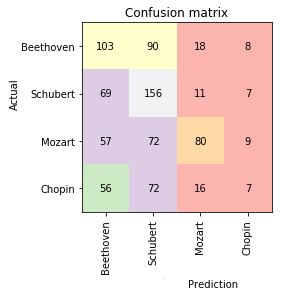
\includegraphics{report/plots/MFCC.png}
\caption{Gaussian NB confusion matrix for MFCC}
Accuracy = 41.63658243080626
\end{figure}

2. Compactness

\begin{figure}[h!]
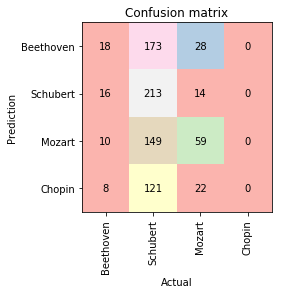
\includegraphics{report/plots/Compact.png}
\caption{Gaussian NB confusion matrix for Compactness}
Accuracy = 34.89771359807461
\end{figure}

3. Spectral Flux

\begin{figure}[h!]
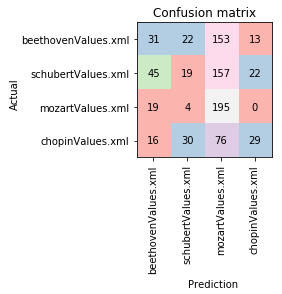
\includegraphics{report/plots/SpectralFlux.png}
\caption{Gaussian NB confusion matrix for Spectral Flux}
Accuracy =
34.89771359807461
\end{figure}


4. Peak Speactral Smoothness

\begin{figure}[h!]
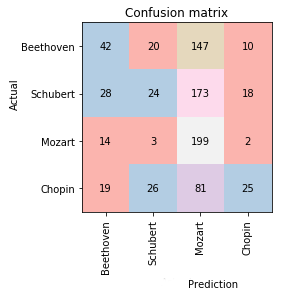
\includegraphics{report/plots/Smooth.png}
\caption{Gaussian NB confusion matrix for Peak Speactral Smoothness}
Accuracy = 34.05535499398315
\end{figure}

5. Method of Moments

\begin{figure}[h!]
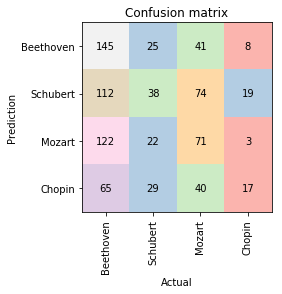
\includegraphics{report/plots/Moments.png}\caption{Gaussian NB confusion matrix for Method of Moments}
Accuracy = 32.61131167268351
\end{figure}


6. Strongest Frequency Via FFT Maximum

\begin{figure}[h!]
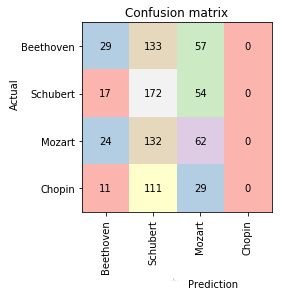
\includegraphics{report/plots/FFTMax.png}
\caption{Gaussian NB confusion matrix for Strongest Frequency Via FFT Maximum}
Accuracy = 31.64861612515042
\end{figure}

7. Root Mean Squared

\begin{figure}[h!]
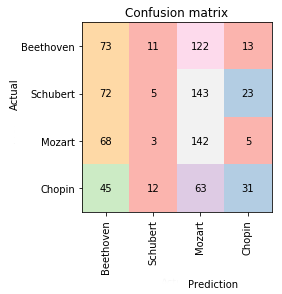
\includegraphics{report/plots/RMS.png} 
\caption{Strongest Frequency Via Root Mean Squared}
Accuracy = 30.20457280385078
\end{figure}

All Features

\begin{figure}[h!]
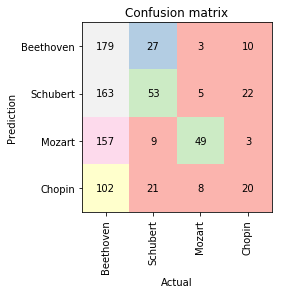
\includegraphics{report/plots/NB_All.png} \caption{Strongest Frequency for All Features}
Accuracy = 36.22141997593261
\end{figure}


From the results it is easy to see that MFCC is a better feature when it
is the only one used versus using all the features. This could be due to
the fact that the data set was not big enough or that some of the
features were not very good choices for distinguishing between different
composers.

    \subsection{Discrete Naïve Bayes}\label{discrete-nauxefve-bayes}

This algorithm used the metadata and message data directly from the MIDI
files to predict the composer of a given piece. The reason for this
implementation was to try and perform the classification with discrete
data straight from the MIDI files in order to avoid inaccuracies and
complications introduced in the processing of the continuous;
multi-dimensional features we extracted using \textbf{jAudio}. Although
it is not a particularly interesting way to view the data (since the
composer of a piece is usually specified in the metadata of a MIDI file)
it may provide an interesting contrast to the other method in terms of
results.

\subsubsection{Implementation Details}\label{implementation-details}

A straightforward implementation of \textbf{Naïve Bayes} with Laplace
smoothing. The features used in this algorithm were extracted directly
from the MIDI files and were chosen for simplicity's sake. Due to
inconsistent labelling of composer names in the MIDI files, some
datapoints got lost in the data preparation process and thus were not
used for this algorithm. Since this algorithm used a different set of
features from the other two, a brief description of these features is
given below:

\paragraph{Key Signature}\label{key-signature}

The first key signature given in the MIDI file. Subsequent key signature
changes were ignored for simplicity. Key signatures are represented as
strings such as \texttt{C} or \texttt{Ab}. Due to inconsistencies in the
representation of key MIDI metadata, some key signatures were
represented twice in two different ways (for example \textbf{F\#} and
\textbf{Gb} which are in fact the same key).

\begin{figure}[htbp!]
\centering
\includegraphics{report/plots/key_freq.png}
\caption{Occurences of different key signatures in the raw MIDI data}
\end{figure}

\paragraph{Time Signature}\label{time-signature}

The first time signature given in the MIDI file. Subsequent time
signature changes were ignored since they are fairly uncommon in the
dataset, and would simply complicate the problem. Time signatures are
represented as strings such as \texttt{3,4} or \texttt{5,4}.

\paragraph{Mean Tempo}\label{mean-tempo}

An average of the tempo throughout the whole piece. This is measured in
ticks. The mean tempo was then discretized by finding the mean \(\mu\)
and variance \(\sigma^2\) of the mean tempos across all data points and
then turning them into discrete values according to the rule:

\(T_{class} = 0 \quad\) if \(T_{value} < \mu - \sigma^2\), Low tempo.

\(T_{class} = 1 \quad\) if
\(\mu - \sigma^2 <= T_{value} <= \mu + \sigma^2\), Mid tempo.

\(T_{class} = 2 \quad\) if \(T_{value} < \mu + \sigma^2\), High tempo.

High mean tempos were absent in the dataset.

\subsubsection{Error On Test Set}\label{error-on-test-set}

When the data was split randomly into training and testing data, one of
the composers tended to be over-represented in the training data,
leading to the model favouring that composer in the prediction. When the
training data was chosen in a favourable way, the results were fairly
good for the two composers case.

\begin{figure}[htbp]
\centering
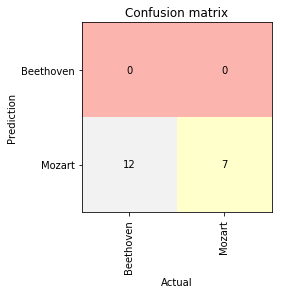
\includegraphics{report/plots/confusion_discNB_01.png}
\caption{Discrete Naïve Bayes on a random test set (two composers).
First result.}
\end{figure}

\begin{figure}[htbp]
\centering
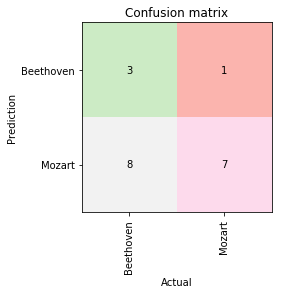
\includegraphics{report/plots/confusion_discNB_01b.png}
\caption{Discrete Naïve Bayes on a random test set (two composers).
Second result.}
\end{figure}

The problem got worse when all four composers were present in the data.
Chopin and Schubert are hugely overrepresented, so the random process
tended to favour them more.

\begin{figure}[htbp]
\centering
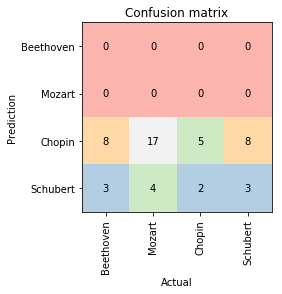
\includegraphics{report/plots/confusion_discNB_02.png}
\caption{Discrete Naïve Bayes on a random test set (four composers).}
\end{figure}

When the number of datapoints for each composer in the training data was
standardized, it improved the results of this algorithm slightly for the
two composers case but didn't improve the results for the four composers
case.

\begin{figure}[htbp]
\centering
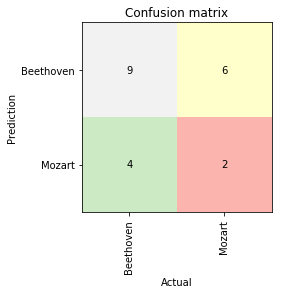
\includegraphics{report/plots/confusion_discNB_03.png}
\caption{Discrete Naïve Bayes on an equalized test set (two composers).}
\end{figure}

\begin{figure}[htbp]
\centering
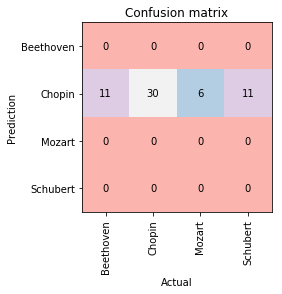
\includegraphics{report/plots/confusion_discNB_04.png}
\caption{Discrete Naïve Bayes on an equalized test set (four
composers).}
\end{figure}

The lack of improvement in the four composers case serves to demonstrate
that either the dataset is too small or these features are not
sufficient to characterise a composer's style and thus are a poor choice
compared to the extracted audio features used in the other algorithms.

    \subsection{Logistic Regression}\label{logistic-regression}

This algorithm used the same data as the \textbf{Gaussian Naïve Bayes}
algorithm. Logistic regression gave us a more discriminative method in
comparison to \textbf{Naïve Bayes} which is more generative. Thus, this
led to a more continuous measure that provides us with a probability
which represents the likelihood that a piano composition belongs to a
certain composer.

\subsubsection{Implementation Details}\label{implementation-details}

We implemented multiclass classification using the ``One vs Rest(OVR)''
method. Since we have 4 target classes, namely; \textbf{Beethoven},
\textbf{Chopin}, \textbf{Mozart} and \textbf{Schubert}, we first treated
\textbf{Beethoven} as one class and \textbf{Chopin}, \textbf{Mozart} and
\textbf{Schubert} as the other class and then ran our logistic
regression model. We repeated this process for each composer and ended
up with 4 different, independent logistic regressions.

We then had 4 classifiers to use for prediction where each one gave us a
probability of its associated class. The most probable class is then the
one that yields the highest probability.

\subsubsection{Hyperparameters}\label{hyperparameters}

The learning rate, \(\alpha\), that we used initially had a value of
0.1. This gave us an accuracy of 49.09747\%. We then incrementally
increased its value by 0.1 and discovered that the accuracy of the model
increased as we approached 1. At \(\alpha\) = 1, the models accuracy was
51.98555\%. Despite \(\alpha\) being relatively large, it did not
produce a sub-optimal set of weights.

\subparagraph{\texorpdfstring{\(\alpha\) =
0.1}{\textbackslash{}alpha = 0.1}}\label{alpha-0.1}

\begin{figure}[htbp]
\centering
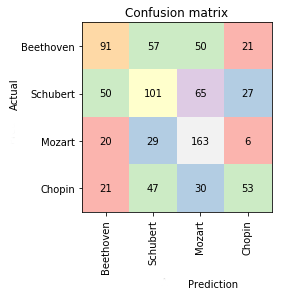
\includegraphics{report/plots/LRalpha1.png}
\caption{Logistic Regression for aplha = 0.1.}
\end{figure}

\subparagraph{\texorpdfstring{\(\alpha\) =
1}{\textbackslash{}alpha = 1}}\label{alpha-1}

\begin{figure}[htbp]
\centering
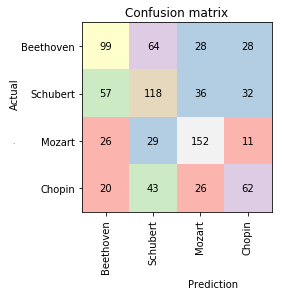
\includegraphics{report/plots/LRalpha2.png}
\caption{Logistic Regression for aplha = 1.0.}
\end{figure}

    \section{Discussion of Results}\label{discussion-of-results}

The \textbf{Gaussian Naïve Bayes} algorithm performed sub-optimally
compared to \textbf{Logistic Regression} but a lot better than
\textbf{Discrete Naïve Bayes}. As stated above, a possible reason for
the poor performance of \textbf{Gaussian Naïve Bayes} is the lack of
data or the fact that some of the extracted features did not correlate
sufficiently.

The \textbf{Discrete Naïve Bayes} algorithm performed the worst by far.
This is most likely due to the limited number of data points and the
lack of readily available features in the MIDI files.

\subsection{Best Possible Performance}\label{best-possible-performance}

\textbf{Logistic Regression} was the best performer out of the 3
algorithms used. The difference in accuracy was approximately 15\%. The
main possible reason for the algorithm performing better is due to the
lack of bias and high variance within our dataset and the algorithms
itself. \textbf{Logistic Regression} was also less computationality
heavy compared to the other algorithms which means it ran a lot quicker.

In conclusion, \textbf{Logistic Regression} performed better than
complete randomness. Thus we were able to predict if certain musical
pieces were composed by \textbf{Beethoven}, \textbf{Chopin},
\textbf{Mozart} and \textbf{Schubert} using the extracted features.

\subsection{Recommendations to Others Working on This
Data}\label{recommendations-to-others-working-on-this-data}

\begin{itemize}
\tightlist
\item
  Don't use the raw MIDI data. Extracting established audio features is
  much more effective.
\item
  Split the compositions into short snippets to increase the size of the
  dataset.
\item
  Avoid audio features that give a huge number of values such as
  \textbf{Power Spectrum} since these will only add to \emph{the curse
  of dimensionality}.
\item
  Make sure to use MFCC as a feature, it seems to be a strong predictor.
\item
  Due to the similarity between composers, this made it more difficult
  for our alrgorithms to properly identify the musical compositions.
  Therefore, choosing composers from different eras of classifical music
  could possibly give a higher accuracy.
\end{itemize}

\newpage

\section{Appendix A}\label{appendix-a}

\subsection{
Description of datapoint after extraction through \textbf{jAudio}}

\texttt{\textless{}section\ start="16.384"\ stop="32.7679375"\textgreater{}\ \ \ \ \ \ \ \ \ \textless{}feature\textgreater{}\ \ \ \ \ \ \ \ \ \ \ \ \ \textless{}name\textgreater{}Spectral\ Flux\textless{}/name\textgreater{}\ \ \ \ \ \ \ \ \ \ \ \ \ \textless{}v\textgreater{}8.51E-6\textless{}/v\textgreater{}\ \ \ \ \ \ \ \ \ \textless{}/feature\textgreater{}\ \ \ \ \ \ \ \ \ \textless{}feature\textgreater{}\ \ \ \ \ \ \ \ \ \ \ \ \ \textless{}name\textgreater{}Compactness\textless{}/name\textgreater{}\ \ \ \ \ \ \ \ \ \ \ \ \ \textless{}v\textgreater{}7.406E5\textless{}/v\textgreater{}\ \ \ \ \ \ \ \ \ \textless{}/feature\textgreater{}\ \ \ \ \ \ \ \ \ \textless{}feature\textgreater{}\ \ \ \ \ \ \ \ \ \ \ \ \ \textless{}name\textgreater{}Spectral\ Variability\textless{}/name\textgreater{}\ \ \ \ \ \ \ \ \ \ \ \ \ \textless{}v\textgreater{}8.891E-6\textless{}/v\textgreater{}\ \ \ \ \ \ \ \ \ \textless{}/feature\textgreater{}\ \ \ \ \ \ \ \ \ \textless{}feature\textgreater{}\ \ \ \ \ \ \ \ \ \ \ \ \ \textless{}name\textgreater{}Root\ Mean\ Square\textless{}/name\textgreater{}\ \ \ \ \ \ \ \ \ \ \ \ \ \textless{}v\textgreater{}1.367E-2\textless{}/v\textgreater{}\ \ \ \ \ \ \ \ \ \textless{}/feature\textgreater{}\ \ \ \ \ \ \ \ \ \textless{}feature\textgreater{}\ \ \ \ \ \ \ \ \ \ \ \ \ \textless{}name\textgreater{}Zero\ Crossings\textless{}/name\textgreater{}\ \ \ \ \ \ \ \ \ \ \ \ \ \textless{}v\textgreater{}1.631E4\textless{}/v\textgreater{}\ \ \ \ \ \ \ \ \ \textless{}/feature\textgreater{}\ \ \ \ \ \ \ \ \ \textless{}feature\textgreater{}\ \ \ \ \ \ \ \ \ \ \ \ \ \textless{}name\textgreater{}Strongest\ Frequency\ Via\ Zero\ Crossings\textless{}/name\textgreater{}\ \ \ \ \ \ \ \ \ \ \ \ \ \textless{}v\textgreater{}4.976E2\textless{}/v\textgreater{}\ \ \ \ \ \ \ \ \ \textless{}/feature\textgreater{}\ \ \ \ \ \ \ \ \ \textless{}feature\textgreater{}\ \ \ \ \ \ \ \ \ \ \ \ \ \textless{}name\textgreater{}Strongest\ Frequency\ Via\ Spectral\ Centroid\textless{}/name\textgreater{}\ \ \ \ \ \ \ \ \ \ \ \ \ \textless{}v\textgreater{}5.82E2\textless{}/v\textgreater{}\ \ \ \ \ \ \ \ \ \textless{}/feature\textgreater{}\ \ \ \ \ \ \ \ \ \textless{}feature\textgreater{}\ \ \ \ \ \ \ \ \ \ \ \ \ \textless{}name\textgreater{}Strongest\ Frequency\ Via\ FFT\ Maximum\textless{}/name\textgreater{}\ \ \ \ \ \ \ \ \ \ \ \ \ \textless{}v\textgreater{}6.594E2\textless{}/v\textgreater{}\ \ \ \ \ \ \ \ \ \textless{}/feature\textgreater{}\ \ \ \ \ \ \ \ \ \textless{}feature\textgreater{}\ \ \ \ \ \ \ \ \ \ \ \ \ \textless{}name\textgreater{}MFCC\textless{}/name\textgreater{}\ \ \ \ \ \ \ \ \ \ \ \ \ \textless{}v\textgreater{}-1.225E2\textless{}/v\textgreater{}\ \ \ \ \ \ \ \ \ \ \ \ \ \textless{}v\textgreater{}1.344E1\textless{}/v\textgreater{}\ \ \ \ \ \ \ \ \ \ \ \ \ \textless{}v\textgreater{}-1.062E1\textless{}/v\textgreater{}\ \ \ \ \ \ \ \ \ \ \ \ \ \textless{}v\textgreater{}-3.897E0\textless{}/v\textgreater{}\ \ \ \ \ \ \ \ \ \ \ \ \ \textless{}v\textgreater{}-3.706E0\textless{}/v\textgreater{}\ \ \ \ \ \ \ \ \ \ \ \ \ \textless{}v\textgreater{}1.668E0\textless{}/v\textgreater{}\ \ \ \ \ \ \ \ \ \ \ \ \ \textless{}v\textgreater{}2.414E0\textless{}/v\textgreater{}\ \ \ \ \ \ \ \ \ \ \ \ \ \textless{}v\textgreater{}2.589E0\textless{}/v\textgreater{}\ \ \ \ \ \ \ \ \ \ \ \ \ \textless{}v\textgreater{}-1.625E0\textless{}/v\textgreater{}\ \ \ \ \ \ \ \ \ \ \ \ \ \textless{}v\textgreater{}3.015E-1\textless{}/v\textgreater{}\ \ \ \ \ \ \ \ \ \ \ \ \ \textless{}v\textgreater{}1.797E0\textless{}/v\textgreater{}\ \ \ \ \ \ \ \ \ \ \ \ \ \textless{}v\textgreater{}1.988E0\textless{}/v\textgreater{}\ \ \ \ \ \ \ \ \ \ \ \ \ \textless{}v\textgreater{}-1.681E-1\textless{}/v\textgreater{}\ \ \ \ \ \ \ \ \ \textless{}/feature\textgreater{}\ \ \ \ \ \ \ \ \ \textless{}feature\textgreater{}\ \ \ \ \ \ \ \ \ \ \ \ \ \textless{}name\textgreater{}LPC\textless{}/name\textgreater{}\ \ \ \ \ \ \ \ \ \ \ \ \ \textless{}v\textgreater{}-9.465E-1\textless{}/v\textgreater{}\ \ \ \ \ \ \ \ \ \ \ \ \ \textless{}v\textgreater{}9.681E-1\textless{}/v\textgreater{}\ \ \ \ \ \ \ \ \ \ \ \ \ \textless{}v\textgreater{}-5.564E-1\textless{}/v\textgreater{}\ \ \ \ \ \ \ \ \ \ \ \ \ \textless{}v\textgreater{}5.075E-1\textless{}/v\textgreater{}\ \ \ \ \ \ \ \ \ \ \ \ \ \textless{}v\textgreater{}-3.432E-1\textless{}/v\textgreater{}\ \ \ \ \ \ \ \ \ \ \ \ \ \textless{}v\textgreater{}3.585E-1\textless{}/v\textgreater{}\ \ \ \ \ \ \ \ \ \ \ \ \ \textless{}v\textgreater{}-1.659E-1\textless{}/v\textgreater{}\ \ \ \ \ \ \ \ \ \ \ \ \ \textless{}v\textgreater{}-2.825E-2\textless{}/v\textgreater{}\ \ \ \ \ \ \ \ \ \ \ \ \ \textless{}v\textgreater{}-3.143E-2\textless{}/v\textgreater{}\ \ \ \ \ \ \ \ \ \ \ \ \ \textless{}v\textgreater{}0E0\textless{}/v\textgreater{}\ \ \ \ \ \ \ \ \ \textless{}/feature\textgreater{}\ \ \ \ \ \ \ \ \ \textless{}feature\textgreater{}\ \ \ \ \ \ \ \ \ \ \ \ \ \textless{}name\textgreater{}Method\ of\ Moments\textless{}/name\textgreater{}\ \ \ \ \ \ \ \ \ \ \ \ \ \textless{}v\textgreater{}2.216E-1\textless{}/v\textgreater{}\ \ \ \ \ \ \ \ \ \ \ \ \ \textless{}v\textgreater{}1.208E4\textless{}/v\textgreater{}\ \ \ \ \ \ \ \ \ \ \ \ \ \textless{}v\textgreater{}1.11E8\textless{}/v\textgreater{}\ \ \ \ \ \ \ \ \ \ \ \ \ \textless{}v\textgreater{}4.405E12\textless{}/v\textgreater{}\ \ \ \ \ \ \ \ \ \ \ \ \ \textless{}v\textgreater{}3.371E17\textless{}/v\textgreater{}\ \ \ \ \ \ \ \ \ \textless{}/feature\textgreater{}\ \ \ \ \ \ \ \ \ \textless{}feature\textgreater{}\ \ \ \ \ \ \ \ \ \ \ \ \ \textless{}name\textgreater{}Partial\ Based\ Spectral\ Centroid\textless{}/name\textgreater{}\ \ \ \ \ \ \ \ \ \ \ \ \ \textless{}v\textgreater{}4.152E1\textless{}/v\textgreater{}\ \ \ \ \ \ \ \ \ \textless{}/feature\textgreater{}\ \ \ \ \ \ \ \ \ \textless{}feature\textgreater{}\ \ \ \ \ \ \ \ \ \ \ \ \ \textless{}name\textgreater{}Partial\ Based\ Spectral\ Flux\textless{}/name\textgreater{}\ \ \ \ \ \ \ \ \ \ \ \ \ \textless{}v\textgreater{}-6.508E-3\textless{}/v\textgreater{}\ \ \ \ \ \ \ \ \ \textless{}/feature\textgreater{}\ \ \ \ \ \ \ \ \ \textless{}feature\textgreater{}\ \ \ \ \ \ \ \ \ \ \ \ \ \textless{}name\textgreater{}Peak\ Based\ Spectral\ Smoothness\textless{}/name\textgreater{}\ \ \ \ \ \ \ \ \ \ \ \ \ \textless{}v\textgreater{}4.624E2\textless{}/v\textgreater{}\ \ \ \ \ \ \ \ \ \textless{}/feature\textgreater{}\ \ \ \ \ \ \ \ \ \textless{}feature\textgreater{}\ \ \ \ \ \ \ \ \ \ \ \ \ \textless{}name\textgreater{}Relative\ Difference\ Function\textless{}/name\textgreater{}\ \ \ \ \ \ \ \ \ \ \ \ \ \textless{}v\textgreater{}-4.923E0\textless{}/v\textgreater{}\ \ \ \ \ \ \ \ \ \textless{}/feature\textgreater{}\ \ \ \ \ \textless{}/section\textgreater{}}

    \begin{Verbatim}[commandchars=\\\{\}]
{\color{incolor}In [{\color{incolor} }]:} 
\end{Verbatim}


    % Add a bibliography block to the postdoc
    
    
    
    \end{document}
